\documentclass[a4paper]{article}
\usepackage[utf8x]{inputenc}
\usepackage[portuguese]{babel}
\usepackage{graphicx}
\usepackage{a4wide}
\usepackage[pdftex,hidelinks]{hyperref}
\usepackage{float}
\usepackage{indentfirst}
\usepackage{subcaption}
\usepackage[cache=false]{minted}
\usepackage{amsmath}
\usepackage{listings}
\usepackage{color}
\usepackage{gensymb}
\usepackage{tikz}

\definecolor{dkgreen}{rgb}{0,0.6,0}
\definecolor{gray}{rgb}{0.5,0.5,0.5}
\definecolor{mauve}{rgb}{0.58,0,0.82}

\lstset{frame=tb,
language=C++,
aboveskip=3mm,
belowskip=3mm,
showstringspaces=false,
columns=flexible,
basicstyle={\small\ttfamily},
numbers=none,
numberstyle=\tiny\color{gray},
keywordstyle=\color{blue},
commentstyle=\color{dkgreen},
stringstyle=\color{mauve},
breaklines=true,
breakatwhitespace=true,
tabsize=4
}

\newcommand{\x}{\times}

\begin{document}

\title{Computação Gráfica\\ Animações}
\author{Bárbara Cardoso (a80453) \and Márcio Sousa (a82400) \and Pedro Mendes (a79003)}
\date{\today}

\begin{titlepage}

    %título
    \thispagestyle{empty}
    \begin{center}
        \begin{minipage}{0.75\linewidth}
            \centering
            %engenharia logo
            
\includegraphics[width=0.4\textwidth]{eng.jpeg}\par\vspace{1cm}
            \vspace{1.5cm}
            %títulos
            \href{https://www.uminho.pt/PT}{\scshape\LARGE Universidade do Minho} \par
            \vspace{1cm}
            \href{https://www.di.uminho.pt/}{\scshape\Large Departamento de Informática} \par
            \vspace{1.5cm}

            \maketitle
        \end{minipage}
    \end{center}

\end{titlepage}

\tableofcontents

\pagebreak

\section{Introdução}
Este trabalho foi proposto no âmbito da unidade curricular de Computação Gráfica, e tem como objetivo desenvolver um motor gráfico genérico para representar objetos a 3 dimensões. Este relatório tem como contexto ambos os relatórios anteriores.

Nesta terceira fase do projeto estendemos as capacidades do motor gráfico anteriormente definido com a adição de animações e de mais opções de camera.

O gerador de modelos foi também estendido para processar \textit{Bezier Patches} de forma a ser mais fácil adicionar modelos complexos sem ser necessário o uso das primitivas.

Por fim, o modelo de teste utilizado (O Sistema Solar) foi alterado para demonstrar estas capacidades, fazendo com que os planetas orbitassem o Sol e com que as luas orbitassem os planetas, contando ainda com a adição de um cometa e de uma cintura de asteroides.

\section{Arquitetura do Projecto}

\subsection{Model}\label{sec:models}

Os modelos passaram a ser desenhados com \textit{Vertex Buffer Objects} (VBOs). Estes permitem reduzir o número de pedidos feitos à placa gráfica, aumentando assim, significativamente, a performance do programa.

Por outro lado, perderam a possibilidade de ser desenhados com todos os seus triângulos pintados de cores aleatórias, visto que não é possível especificar a cor de cada triângulo quando estes são todos enviados para o GPU simultaneamente.

Esta desvantagem irá, no entanto, ser mitigada na próxima fase com a adição de luz e texturas.

\subsection{Transformations}

Para que fosse possível animar os modelos, para cada transformação foi criada uma nova versão \textit{animada}: \texttt{TranslateAnimated}~(\ref{sec:translate}), \texttt{RotateAnimated}~(\ref{sec:rotate}), \texttt{ScaleAnimated}~(\ref{sec:scale}).

Todas estas recebem o tempo que demoram a completar a animação. Quando uma animação termina recomeça imediatamente.

\subsubsection{TranslateAnimated}\label{sec:translate}

Esta transformação recebe um conjunto de pontos que definem um caminho pelo qual o modelo deve viajar.

Depois, fazendo uso do número de milissegundos que já passaram desde o início do programa, calcula, usando o algoritmo de \textit{Catmul-Rom}, o ponto no caminho em que o modelo deve estar para esse milissegundo.

\subsubsection{RotateAnimated}\label{sec:rotate}

A rotação animada, ao contrário da sua versão estática, recebe uma duração em vez de receber um ângulo, mantendo os outros parâmetros. Esta duração é mais tarde usada para determinar quanto tempo demora o objeto a efetuar uma rotação de 360\degree{} graus.

Depois, simplesmente calcula um ângulo a partir do tempo que passou desde o início do programa para determinar o ângulo para esse instante.

\begin{figure}[H]
    \[
        angle = \frac{elapsed \x 360}{duracao}
    \]
    \caption{Formula de calculo do ângulo da rotação para um dado instante}
\end{figure}

\subsubsection{ScaleAnimated}\label{sec:scale}

A escala animada adiciona aos antigos rácios para $x, y, z$ um novo triplo de rácios, e para animar vai, simplesmente, ``progredindo'' de um rácio para outro durante o tempo que a animação demora. Sendo que, no início e no fim da animação se encontra no primeiro triplo.

\begin{figure}[H]
    \[
        t = |2 \x \frac{elapsed}{dur} - 1|\\
    \]
    \[
        R = (x_i + t (x_f - x_i), y_i + t (y_f - y_i), z_i + t (z_f - z_i))
    \]
    \caption{Formula usada para determinar o rácio $R$ da animação para o instante $elapsed$.}
\end{figure}

\subsubsection{Group}

O método de desenho recebe agora o tempo que passou desde o início do programa, para que o possa passar às várias transformações, assegurando assim que todas usam o mesmo valor de tempo.

\subsection{\textit{Follow mode}}

Neste momento os models deslocam-se, o que torna mais complicado de os ver. Assim, para resolver este problema
foi implementado o \textit{Follow mode}. Neste o utilizador pode escolher um \textit{model}
para a câmara seguir. Sendo que, o comportamento da câmara neste modo é igual ao antigo
\textit{explorer mode} apenas com a diferença do centro, em que no modo antigo era na origem do referencial e agora passou a ser objeto.

Para conseguir este efeito, foram feitas duas grandes alterações fundamentais aos módulos \textit{Group} e \textit{Câmara}.

\subsubsection{Group}

Para poder focar a câmara no objeto é necessário obter a sua posição no espaço 3D. O problema com este requisito é que os \textit{models} em si não têm coordenadas próprias, são transladados, rodados e escalados para as suas posições. Logo, é necessário que o \textit{Group} tenha a capacidade de calcular as coordenadas de cada modelo.

Para este fim, foi implementado um método que dado um índice vai multiplicando todas as matrizes de transformação até chegar ao modelo, e por fim usa a matriz final para extrair as coordenadas do modelo.

\begin{figure}[H]
    \centering
    \usetikzlibrary{matrix,backgrounds,positioning,calc,fit}
\definecolor{SceneColor}{RGB}{200,200,200}
\definecolor{GroupColor}{RGB}{90,200,102}
\definecolor{SubGroupColor}{RGB}{114,247,247}

\begin{tikzpicture}[font=\ttfamily,
    array/.style={matrix of nodes,
    nodes={draw, minimum width=16mm, minimum height=5mm, fill=white},
    column sep=-\pgflinewidth,
    row sep=-\pgflinewidth,
    nodes in empty cells,
    row 1/.style={nodes={draw=none, fill=none, minimum size=5mm}}}]

    \matrix[array] (Scene) {
        & Scene & \\
        &  &    \\
    };

    \matrix[array, below = of Scene] (Group2) {
        Group 2 \\
        Model 4 & Model 5 \\
        \\
    };

    \matrix[array, left = of Group2] (Group1) {
        &  Group 1 & \\
        Model 1 & Model 2 & Model 3 \\
    };

    \matrix[array, right = of Group2] (Group3) {
        Group 3 \\
        Model 7 \\
    };

    \matrix[array, below = of Group2] (Group21) {
        Group 2.1 \\
        Model 6 \\
    };

    \node[draw, fill=GroupColor, minimum size=2mm, circle] at (Scene-2-1) (Group1Ball) {};
    \node[draw, fill=GroupColor, minimum size=2mm, circle] at (Scene-2-2) (Group2Ball) {};
    \node[draw, fill=GroupColor, minimum size=2mm, circle] at (Scene-2-3) (Group3Ball) {};
    \node[draw, fill=SubGroupColor, minimum size=2mm, circle] at (Group2-3-1) (Group21Ball) {};

    \begin{scope}[on background layer]
        \node[draw, fill=SceneColor, fit = (Scene) (Group1) (Group2) (Group3) (Group21)]
        (SceneBox) {};
        \node[draw, fill=GroupColor, fit = (Group1)] (Group1Box) {};
        \node[draw, fill=GroupColor, fit = (Group2) (Group21)] (Group2Box) {};
        \node[draw, fill=GroupColor, fit = (Group3)] (Group3Box) {};
        \node[draw, fill=SubGroupColor, fit = (Group21)] (Group21Box) {};
    \end{scope}

    \foreach \from/\to in {
        Group1Ball/Group1Box, Group2Ball/Group2Box,
        Group3Ball/Group3Box, Group21Ball/Group21Box}
    \draw [->, thick] (\from)--(\to);

\end{tikzpicture}

    \caption{Representação gráfica da numeração dos modelos}
\end{figure}

\subsubsection{Câmara}

A câmara, por outro lado, sofreu uma grande reestruturação do seu antigo modo \textit{Explorer}.
Foi então concluído que o \textit{Follow mode} era o caso geral deste, ou seja, o \textit{Explorer mode}
permitia ao utilizador focar-se na origem enquanto se deslocava na superfície de uma esfera (invisível), podendo-se alterar o raio desta esfera. Por outro lado, o \textit{Follow mode} permite
ao utilizador fazer tudo isto, mas focando-se em qualquer ponto do espaço 3D. Desta forma, o \textit{Explorer mode} foi substituído pelo novo, \textit{Follow mode}.

\section{Generator}

Uma nova funcionalidade foi adicionada ao \texttt{generator}. Este é agora capaz de ler \textit{patch files} que definem superfícies \texttt{Bezier} e transforma-los nos ficheiros \texttt{.3d} que o \texttt{engine} está preparado para receber.

Um \textit{patch file} contém duas secções: \textit{patches} e pontos de controlo.

Os pontos de controlo contém triplos de coordenadas que irão ser usados pelos \textit{patches}, enquanto que os \textit{patches} contêm um \textit{patch} por linha.

\subsection{Patch}

Um \textit{patch} é um conjunto de 16 pontos que definem uma superfície de Bezier (cada linha contém, na verdade, 16 índices que referenciam os pontos de controlo da superfície).

Cada patch destes representa uma superfície e os 16 pontos são divididos em grupos de 4 que descrevem arcos desta superfície. Depois, para cada arco definem-se os pontos da curva usando o nível de \textit{tessellation} para definir quantos pontos criar. Por fim, utilizando estes pontos aplica se o mesmo algoritmo para definir N curvas (uma para cada 4 pontos de cada arco) unindo os 4 arcos e formando uma rede de arcos. Os quadrados desta rede são mais tarde partidos em dois triângulos e serializados como 6 pontos no espaço.

\begin{figure}[H]
    \centering
    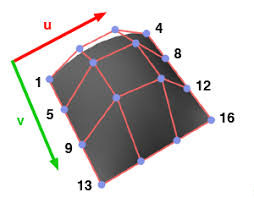
\includegraphics[width=0.3\textwidth]{bezier.jpg}
    \caption{A superfície gerada por pontos de controlo}
\end{figure}

\section{Alterações dos ficheiros de input}\label{sec:estrutura-ficheiros}

O \texttt{XML} de input utilizado foi estendido para possibilitar a utilização das novas funcionalidades, no entanto, foi mantida a \textit{backwards compatibility} para o formato anterior. De forma a que modelos antigos continuem a ser validos. Uma ligeira diferença, no entanto, é que o parâmetro \texttt{RAND} agora apenas define um cor aleatória para o grupo, ao contrario do comportamento anterior em que desenhava todos os triângulos de todos os seus modelos de cor diferente (ver secção~\ref{sec:models})

\subsection{Translação Animada}

Para definir uma translação animada cria-se um bloco \textit{translate} com o parâmetro \texttt{TIME}, e dentro deste define se a lista de pontos que a translação ira seguir.

Por exemplo:
\begin{minted}{xml}
    <translate time="1" >
        <point X="1" Y="1" Z="1"/>
        <point Y="1" />
        <point Z="1" />
        <point X="1.4" />
    </translate>
\end{minted}

Todos os parâmetros podem ser omitidos, pois todos tem valores por defeito: 0 para as coordenadas dos pontos, e 1 para a duração da animação.

\subsection{Rotação Animada}

Uma rotação animada troca apenas o ângulo por uma duração.
\begin{minted}{xml}
    <rotate X="1" TIME="1" />
\end{minted}

Tal como na translação todos os parâmetros podem ser omitidos, com excepção da duração, que é usada para determinar se a rotação é estática ou animada.

\subsection{Escala Animada}

Uma escala animada tem de receber a escala inicial e a escala final, denominada no \texttt{XML} como \texttt{XI, YI, ZI} e \texttt{XF, YF, ZF} respectivamente. Junto destas espera também uma parâmetro \texttt{time} para a duração.

\begin{minted}{xml}
    <scale XI="20" YI="20" ZI="20" XF="30" YF="30" ZF="30" TIME="1"/>
\end{minted}

Todos estes tem valores por defeito e podem ser omitidos.

\section{Key Bindings}

Novas \textit{key bindings} foram adicionadas:

\begin{itemize}
    \item \texttt{Shift+I} e \texttt{Shift+O}: Similares ao \texttt{I} e
        \texttt{O} permitem diminuir e aumentar o raio do \textit{Follow mode},
        mas a uma velocidade mais alta.
    \item \verb!{! e \verb!}!: Permite seleccionar o modelo a seguir.
    \item \texttt{,}: Liga/Desliga as rotas dos modelos em translação.
    \item \verb!(! e \verb!)!: Aumenta e Diminui a velocidade com que o tempo
        passa.
    \item \texttt{P}: Liga/Desliga pausa.
\end{itemize}

\section{Sistema Solar}

No Sistema Solar cada um dos astros tem a sua própria órbita e esta é animada, à excepção do sol obviamente.
As órbitas dos planetas são órbitas elípticas, tentando assim retratar o sistema solar real. As órbitas das luas de cada planeta são órbitas circulares com inclinações aleatórias.

Além destes astros, foi adicionado também ao sistema solar uma cintura de asteróides que se situa entre Marte e Júpiter e um cometa com uma órbita elíptica muito alongada. O cometa tem a forma de \textit{teapot} para demonstrar também as capacidades do gerador.

\section{Conclusões e Trabalho Futuro}

Em suma, todas as funcionalidades pedidas foram implementadas assim como alguns extras. No entanto, algumas optimizações não foram implementadas, como por exemplo, o uso de índices no VBOs. Tencionamos adicionar isto na próxima fase.

\end{document}
